\documentclass[10pt]{beamer}
\usepackage{amsmath}
\usefonttheme{professionalfonts} % using non standard fonts for beamer
\usefonttheme{serif} % default family is serif\
\usepackage{mathtools}
%\documentclass[12pt]{beamerthemeSam.sty}
\usepackage{epsf}
\usepackage{ulem}
\usepackage{array}
%\usepackage{pstricks}
%\usepackage[orientation=portrait,size=A4]{beamerposter}
\geometry{paperwidth=160mm,paperheight=120mm}
%DT favorite definitions
\def\LL{\left\langle}   % left angle bracket
\def\RR{\right\rangle}  % right angle bracket
\def\LP{\left(}         % left parenthesis
\def\RP{\right)}        % right parenthesis
\def\LB{\left\{}        % left curly bracket
\def\RB{\right\}}       % right curly bracket
\def\PAR#1#2{ {{\partial #1}\over{\partial #2}} }
\def\PARTWO#1#2{ {{\partial^2 #1}\over{\partial #2}^2} }
\def\PARTWOMIX#1#2#3{ {{\partial^2 #1}\over{\partial #2 \partial #3}} }

\def\rightpartial{{\overrightarrow\partial}}
\def\leftpartial{{\overleftarrow\partial}}
\def\diffpartial{\buildrel\leftrightarrow\over\partial}

\def\BI{\begin{itemize}}
\def\EI{\end{itemize}}
\def\BE{\begin{displaymath}}
\def\EE{\end{displaymath}}
\def\BEA{\begin{eqnarray*}}
\def\EEA{\end{eqnarray*}}
\def\BNEA{\begin{eqnarray}}
\def\ENEA{\end{eqnarray}}
\def\EL{\nonumber\\}
\def\BS{\bigskip}
\def\BC{\begin{center}}
\def\EC{\end{center}}
\def\BCC{\begin{columns}}
\def\ECC{\end{columns}}
\def\HC{\column{0.5\textwidth}}
\newcommand{\etal}{{\it et al.}}
\newcommand{\gbeta}{6/g^2}
\newcommand{\la}[1]{\label{#1}}
\newcommand{\ie}{{\em i.e.\ }}
\newcommand{\eg}{{\em e.\,g.\ }}
\newcommand{\cf}{cf.\ }
\newcommand{\etc}{etc.\ }
\newcommand{\atantwo}{{\rm atan2}}
\newcommand{\Tr}{{\rm Tr}}
\newcommand{\dt}{\Delta t}
\newcommand{\op}{{\cal O}}
\newcommand{\msbar}{{\overline{\rm MS}}}
\def\chpt{\raise0.4ex\hbox{$\chi$}PT}
\def\schpt{S\raise0.4ex\hbox{$\chi$}PT}
\def\MeV{{\rm Me\!V}}
\def\GeV{{\rm Ge\!V}}

%AB: my color definitions
%\definecolor{mygarnet}{rgb}{0.445,0.184,0.215}
%\definecolor{mygold}{rgb}{0.848,0.848,0.098}
%\definecolor{myg2g}{rgb}{0.647,0.316,0.157}

\definecolor{A}{rgb}{0.8,0.0,0.0}
\definecolor{B}{rgb}{0.0,0.6,0.0}
\definecolor{C}{rgb}{0.4,0.4,0.0}
\definecolor{D}{rgb}{0.0,0.0,0.5}
\definecolor{E}{rgb}{0.4,0.4,0.4}


\definecolor{abtitlecolor}{rgb}{0.0,0.255,0.494}
\definecolor{absecondarycolor}{rgb}{0.0,0.416,0.804}
\definecolor{abprimarycolor}{rgb}{1.0,0.686,0.0}
\definecolor{Red}           {cmyk}{0,1,1,0}
\definecolor{Grey}           {cmyk}{.5,.5,.5,0}
\definecolor{Lg}           {cmyk}{.4,.4,.4,0}
\definecolor{Blue}          {cmyk}{1,1,0,0}
\definecolor{Green}         {cmyk}{1,0,1,0}
\definecolor{Brown}         {cmyk}{0,0.81,1,0.60}
\definecolor{Black}         {cmyk}{0,0,0,1}

\usetheme{Madrid}
\setbeamercolor{title}{fg=abtitlecolor}
\setbeamercolor{frametitle}{fg=abtitlecolor}
\setbeamercolor{palette tertiary}{fg=white,bg=abtitlecolor}
\setbeamercolor{palette secondary}{fg=white,bg=absecondarycolor}
\setbeamercolor{palette primary}{fg=black,bg=abprimarycolor}
\setbeamercolor{structure}{fg=abtitlecolor}

\setbeamerfont{section in toc}{series=\bfseries}

%AB: remove navigation icons
\beamertemplatenavigationsymbolsempty
\title{
  \textbf {Torque and rotational dynamics}\\
%\centerline{}
%\centering
%\vspace{-0.0in}
%\includegraphics[width=0.3\textwidth]{propvalues_0093.pdf}
%\vspace{-0.3in}\\
%\label{intrograph}
}

\author[W. Freeman] {Physics 211\\Syracuse University, Physics 211 Spring 2022\\Walter Freeman}

\date{\today}

\begin{document}

\frame{\titlepage}


\frame{\frametitle{\textbf{Announcements}}
\Large

I'm back! (Thanks, Pfizer/BioNTech!)

\BS\pause

\normalsize

\BI
\item Homework 8 is due tomorrow in recitation (both the new problems and the exam re-do)
\item Remember:
\BI
\item All of our homework is designed as an opportunity for you to {\it learn things}
\item If you're not able to finish understanding everything by the due date, should you:
\BI
\item {\bf A:} Contact Walter and ask for an extension
\item {\bf B:} Contact your TA and ask for an extension
\item {\bf C:} Half-ass something and turn it in anyway; it's due when it's due
\item {\bf D:} Copy someone else's solutions
\EI
\item {\bf We want you to understand this material} -- please ask questions here/on Discord/to your classmates/in the Clinic!
\EI
\EI
}


\frame{\frametitle{\textbf{Announcements}}
	\large
	We will have one more homework assignment after this one.
	
	\BS
	
	It will be due on the last day of the semester, May 3. It will be somewhat long.
	
	\BS
	
	This Friday I will send out a poll about {\it missed exams} and other ``behind on work''  issues. Please make sure you answer it.
}


\frame{\frametitle{\textbf{Final exam conflicts}}
\Large

If your final exam for another class is scheduled at the same time as this one (economics, human sexuality):

\large

\BI
\item Take your final exam for your other class
\item Take an hour for dinner
\item Come to the Physics Clinic at 6pm for your physics exam
\EI
}

\frame{\frametitle{\textbf{Today's agenda}}
\large
\BI
\item Finish our discussion from before, talking about static equilibrium
\item Talk about what is required for an object to balance on a surface
\item Have the professor walk the plank, like the scurvy dog that he is (arr)
\BS\pause
\item Talk about rotational dynamics:
\BI
\item One problem where one object translates and another object rotates
\item One problem where one object both translates and rotates
\EI
\EI
}





\frame{

\Large
\BC
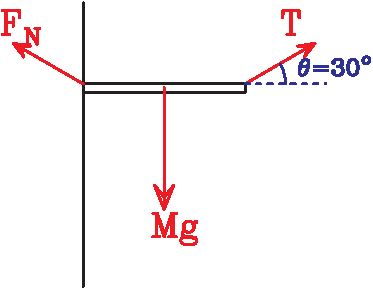
\includegraphics[width=0.5\textwidth]{beam-crop.pdf}

How does the tension $T$ compare to the weight of the beam?

\EC

\BS
\huge
\BCC
\HC
\color{A}A: $T \leq Mg/2$ \\
\color{B}B: $Mg/2 < T < Mg$ \\
\HC
\color{C}C: $T = Mg$ \\
\color{D}D: $Mg < T < 2Mg$ \\
\ECC
\BC
\color{E}E: $T >= 2Mg$ \\
\EC
}

\frame{
\Large

How will the required tension to support the beam change if I walk to the side? (See demo.)

\BS\BS\pause

How will the required tension to support the beam change if I lift my hand? (See demo.)

\BS\BS\pause

What force must the hinge apply to the beam?

}

%
%\frame{\frametitle{\textbf{Balancing objects: will it topple?}}
%
%\large
%
%If an object extends out past the end of a support like the table, how do you know if it will fall?
%
%\BS
%
%Suppose an object extends off the right side of the table.
%
%\BI
%\item Choose the pivot point to be the right edge of the table
%\item Recall that normal forces can only push, never pull
%\item The torque from the table must be clockwise
%\EI
%
%\pause
%\BS
%This suggests the following strategy to see if something will fall or not:
%
%\BI
%\item Choose the pivot point at the right edge of the table
%\item Write down $\sum \tau = 0$, with $\tau_{\rm table}$ as an unknown
%\item Solve for the necessary value of $\tau_{\rm table}$ to keep the object in equilibrium ($\sigma \tau = 0$)
%\item If  $\tau_{\rm table}$ is clockwise, it can stay balanced; if  $\tau_{\rm table}$ is counterclockwise it must fall
%\EI
%
%\pause
%\BS
%Another way to say this: {\it the object begins to fall when the sum of the torques around the edge, from everything {\color{Red}other than the table}, is zero}.
%
%}
%
%\frame{\frametitle{\textbf{Walking the plank}}
%
%\Large
%
%\BC
%How far out can I stand before I fall?
%\EC
%}

\frame{

\Large

Which will make the hanging object fall faster?

\BS

\color{A}A: Increasing the diameter of the spool the string is wound around \\
\color{B}B: Decreasing the diameter of the spool the string is wound around \\
\color{C}C: Moving the spinning masses inward \\
\color{D}D: Moving the spinning masses outward \\
\color{E}E: None of the above; it falls at $g$ no matter what
}


\frame{\frametitle{\textbf{Solving problems with both translation and rotation}}

\Large

Recall how you solved problems back in Unit 2:

\large
\BI
\item Write down force diagrams for everything
\item Construct $\sum \vec F = m \vec a$ for everything
\item This will generate a system of equations
\item Determine constraints (often the accelerations are related: $a_{1,y} = -a_{2,y}$, etc.
\item Solve the system of equations
\EI

\BS
\BS

How does this change now?

\pause


\color{Green}
\BI
\item You also need $\sum \tau = I \alpha$ for objects that rotate
\item This means you need {\color{Red}extended force diagrams} for them to determine $\sum \tau$
\item Often now you will have different kinds of constraints: $a = \pm \alpha r$...
\item If one object both translates and rotates (for instance, if it rolls), you need both $\sum \vec F=m\vec a$ and $\sum \tau = I \alpha$ for it
\EI

\color{Black}

That's it!
}

\frame{\frametitle{\textbf{How fast will the hanging mass fall?}}

\Large

A string is wound around a light pulley at radius $r$. Two brass weights of mass $M$ are at either end of a 
bar attached to the pulley.

\BS

A mass $m$ hangs from the string. How fast does it fall?

}

\frame{\frametitle{\textbf{The Ping-Pong ball on a table}}

\Large

A Ping-Pong ball of mass $m$ rests on a table. The coefficient of static friction between the ball and the table is $\mu_s$.

\BS

(Since the ball is a hollow shell, its moment of inertia is $I = \frac{2}{3}mr^2$.)
\BS

The wind starts to blow, exerting a force $F_w$ on the ball from one side, directed uniformly across the ball.
\pause

\BS

If the wind blows gently, the ball will roll without slipping. If the wind blows more strongly, the ball will
begin to skid along the table.

\BS

What is the maximum value of $F_w$ so that the ball rolls without slipping?

}

\end{document}
